% Document class report-template accepts either: project-plan or final-report option
\documentclass[project-plan]{report-template}

% Packages I want to use in my report.
\usepackage{graphicx}
\usepackage{amsmath}
\usepackage{blindtext}

% Directory where I save my figures.
\graphicspath{{./figures/}}

% Metadata used for the title page.
\university{Imperial College London}
\department{Department of Earth Science and Engineering}
\course{MSc in Applied Computational Science and Engineering}
\title{Forecasting induced seismicity in Oklahoma}
\author{Zhiyong Liu}
\email{zl1220@ic.ac.uk}
\githubusername{acse-liuzyon}
\supervisors{Dr. Stephen P. Hicks}
\repository{https://github.com/acse-2020/acse2020-acse9-projectplan-liuzyon}

\begin{document}

\maketitlepage  % generate title page
\githubrepo  % GitHub repository

% Abstract
\section*{Abstract}

% Introduction section
\section{Introduction}
It is well known that humans can cause earthquakes through fluid injection and extraction.
Fluid injection includes wastewater disposal and hydraulic fracturing, while fluid extraction includes oil, gas and groundwater.
Such cases of induced seismicity have been recorded and proven in Oklahoma, where seismicity has been increased dramatically since 2010 \citep{ellsworth2013injection}.
In cases like Oklahoma, because the rate of earthquakes was very low before high-rate wastewater injection, it is relatively easy to determine the fundamental causes of induced seismicity.
Therefore, due to the low background stress in intraplate regions, the human triggering signatures are clearly identifiable.
However, in tectonically-active areas, it is more challenging to distinfuish between natural and triggered seismicity.
Big-data and statistical approaches will be crucial in separating natural causes from potential human triggering factors in these areas.
Besides, large-scale big-data and statistical approaches are effecient method to predict the locations where human triggered seismicity may be expected.

\section{Literature Review}
Ellsworth stated the current understanding of the causes and mechanics of human-induced earthquakes. It includes wastewater injection, emerging oil and gas recovery technologies, and other indirect induced activities,
including deep fluid injection \citep{ellsworth2013injection}.
Hincks et al. developed a Bayesian network to for quantitative evaulation of correlations between well operational parameters, geological formation, and seismicity.
The injection depth relative to crystalline basement was found to be the most significant parameter for seismic moment release \citep{hincks2018oklahoma}.
Wozniakowska and Eaton performed a machine learning estimation of the seismogenic activation potential for each well using logistic regression and found that the injection depth influence greatly the seismogenic activation potential \citep{wozniakowska2020machine}.
Norbeck and Rubinstein genreated a model based on fluid flow and seismic physics, which associate the past injection trends with the seismicity patterns \citep{norbeck2018hydromechanical}.

The correlations of induced earthquakes with fluid extraction and injection are well established. 
Some physics models are also developed in previous research for earthquake prediction.
However, these researches do not explain why seismicity does not always occured close to an injection well.
Also, these studies did not develop a statistical model or a machine-learning model to predict earthquakes based on well documented data (such recorded data in Oklahoma)

\section{Description of Problem and Objectives}
Although a causal relationship has been established between fluid injection and earthquakes, it is still not known why some areas are more susceptible to induced earthquakes and why seismicity does not always occur close to an injection well. 
To solve these problems, statistical methods and machine learning methods are required.
In this project, a unique and rich dataset of industrial activities from regions in Oklahoma will be used to statistically evaluate and retrospectively forecast possible signatures of human-induced seismicity from existing high-quality earthquake in these regions.
The database used contains well locations, geological metadata, monthly injection and extration volumes. 
To test the existence of correlations of humen induced parameters with seismicity and predict the earthquake occurrences, some machine learning techniques will be developed to generate a model with predictive capabilities.
Linear Regression and logistic Regression will be performed as one starting point to produce a simple model of earthquake occurence. 
Other supervised and unsupervised technologies will also be implemented to obtain the higher performance model.
The main program will be coded in python, including using specific Python libraries such as Pandas, Scikit-Learn, statsmodels, matplotlib and some GIS modules.

\section{Progress to Date and Future Plan}
\begin{figure}
    \begin{center}
        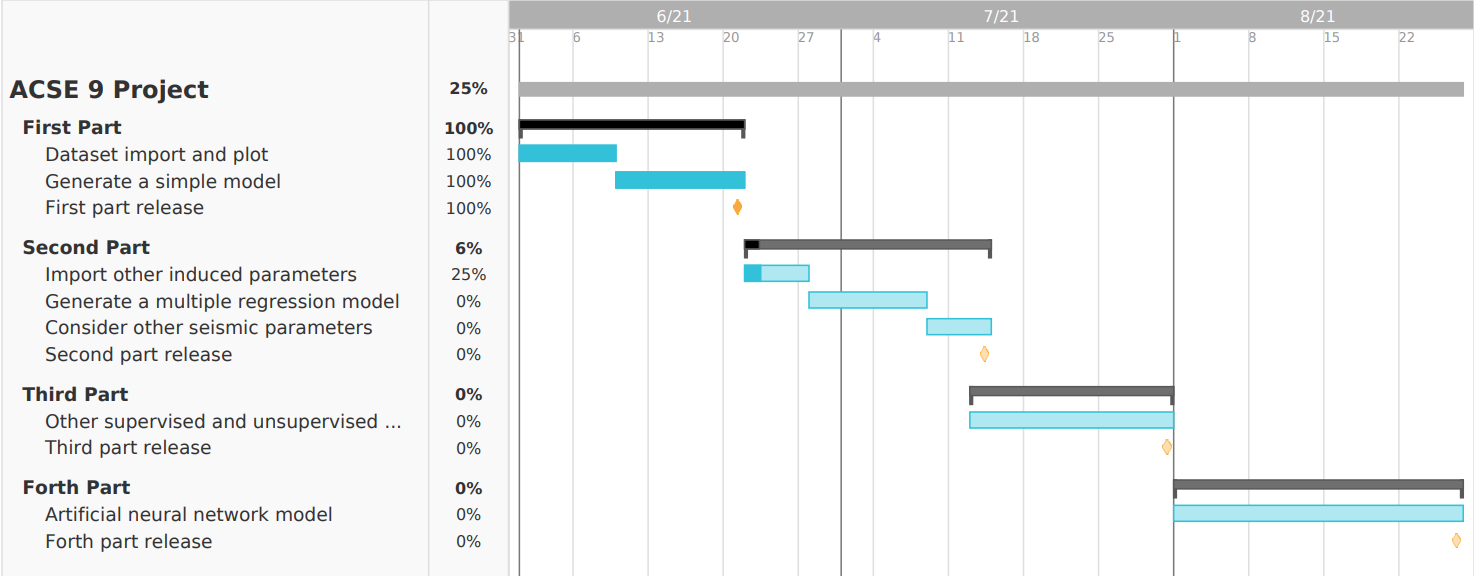
\includegraphics[width=1\textwidth]{gantt.png}
    \end{center}
    \caption{\label{fig:gantt} Gantt chart.}
\end{figure}
In this project, there are many potential parameters to investigate correlations with earthquake activity, which are injection volume, well depth and geological formation being injected into.
The parameters of earthquake activity considered are earthquake occurence, maximum earthquake magnitude and earthquake moment rate.
As Figure~\ref{fig:gantt} shown, This project is divided into four parts.
In the first part, dataset is successfully imported and plotted with geopandas. Then, as a starting point, injection volume will be concentrated on to find the correlation with the earthquake occurence and produce a simple model. 
Here, some regression techniques such as linear or logistic regression will be used for the model generateing.
In the second part, other potential parameters like well depth and geological formation (sedimentary basin thickness, and geological faults) will be introduced to consider together and multiple regression models will be generated.
Besides, other earthquake activity parameters (maximum earthquake magnitude and earthquake moment rate) will also be investigated correlations with induced potential parameters.
In the third part, Other supervised and unsupervised technologies (K-means, PCA, etc.) will be used on the dataset to generate better models compared with linear regression and logistic regression.
In the final part, Deep learning technologies such as Neural network models will be trained with all potential parameters and generated with predictive capabilities.

The development model used in this project is iterative model \citep{alshamrani2015comparison}. In each part, requirements analysis, design, coding, testing will be carried out.
Each iteration will result in a model which can be used to predict. As is demonstrated in the Figure~\ref{fig:gantt}, Each part will generate available models.
For each generated model, a lot of evaluation criterions will be used to test predictive capability, such as MSE, RMSE, MAE, accuracy, confussion matrix, precision, recall and so on. 

The datasets used for this project are extremely huge and varied. They are split into training dataset and testing dataset for generating models and testing.
The preliminary main part of them are wells and earthquakes, which are mapped and shown in Figure~\ref{fig:well} and Figure~\ref{fig:earthquake}. 
Other data such as injection volume and geological formation are also provided in csv and xlsx format.
% \begin{figure}
%     \begin{center}
%         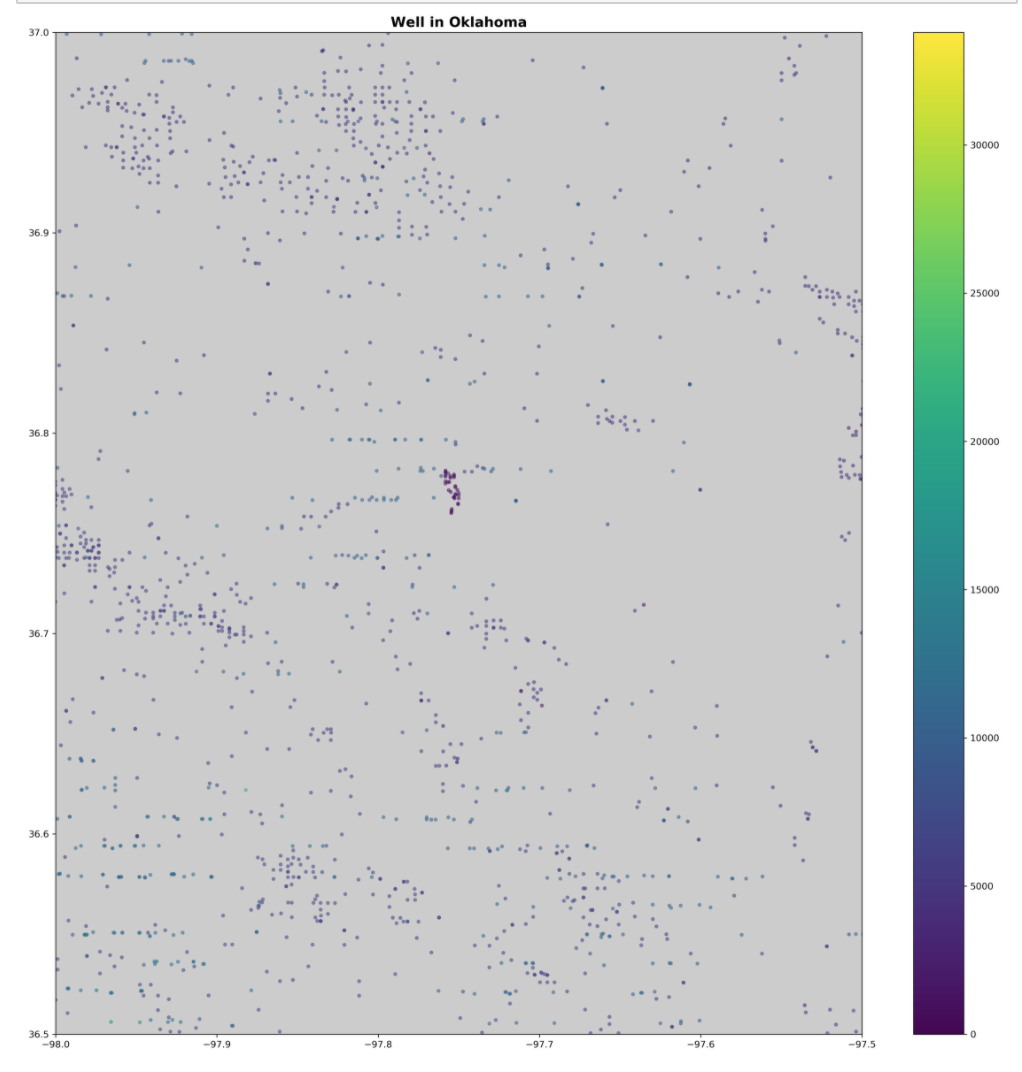
\includegraphics[width=0.5\textwidth]{well.png}
%     \end{center}
%     \caption{\label{fig:well} Well Depth in Oklahoma.}
% \end{figure}

% \begin{figure}
%     \begin{center}
%         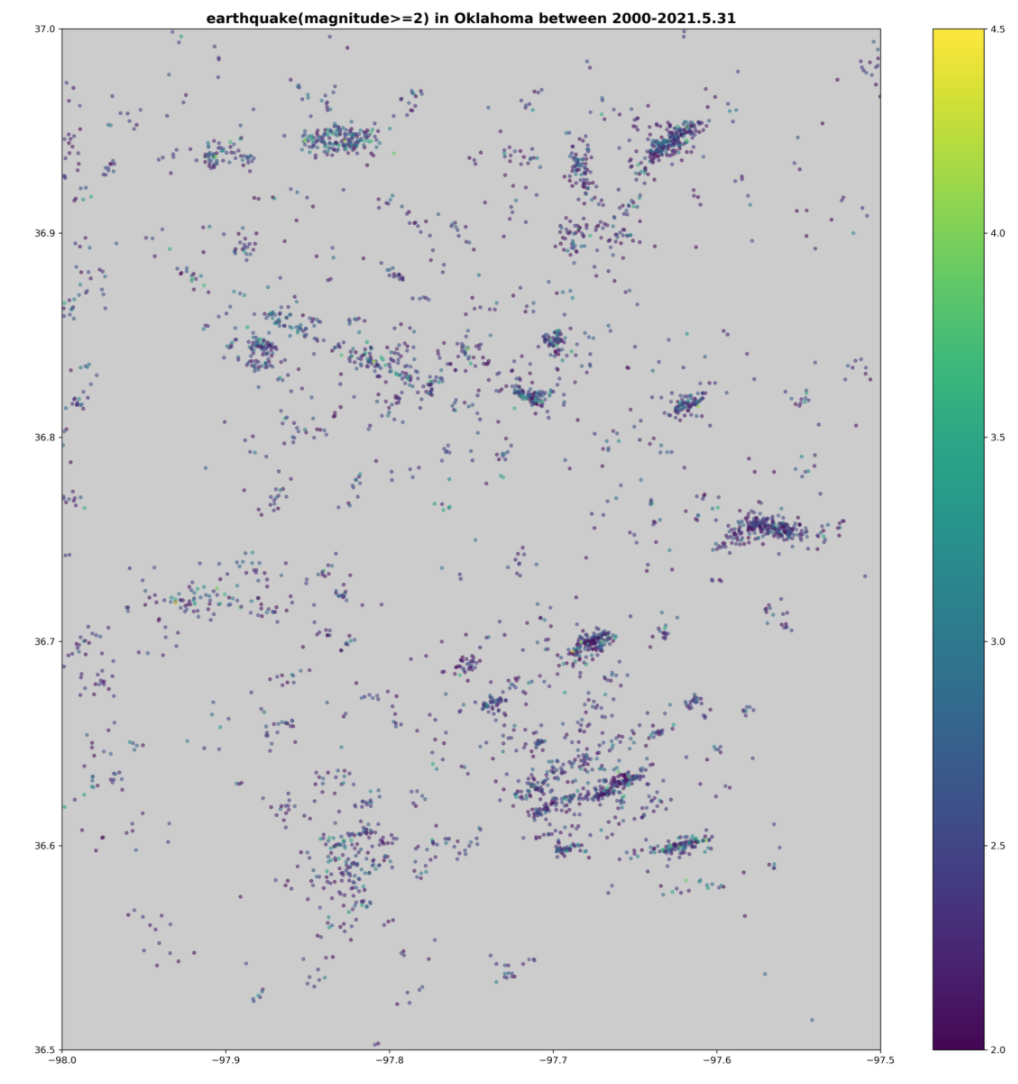
\includegraphics[width=0.5\textwidth]{earthquake.png}
%     \end{center}
%     \caption{\label{fig:earthquake} Earthquake Magnitude in Oklahoma.}
% \end{figure}

\begin{figure}
    \begin{minipage}[t]{0.5\linewidth}
      \centering
      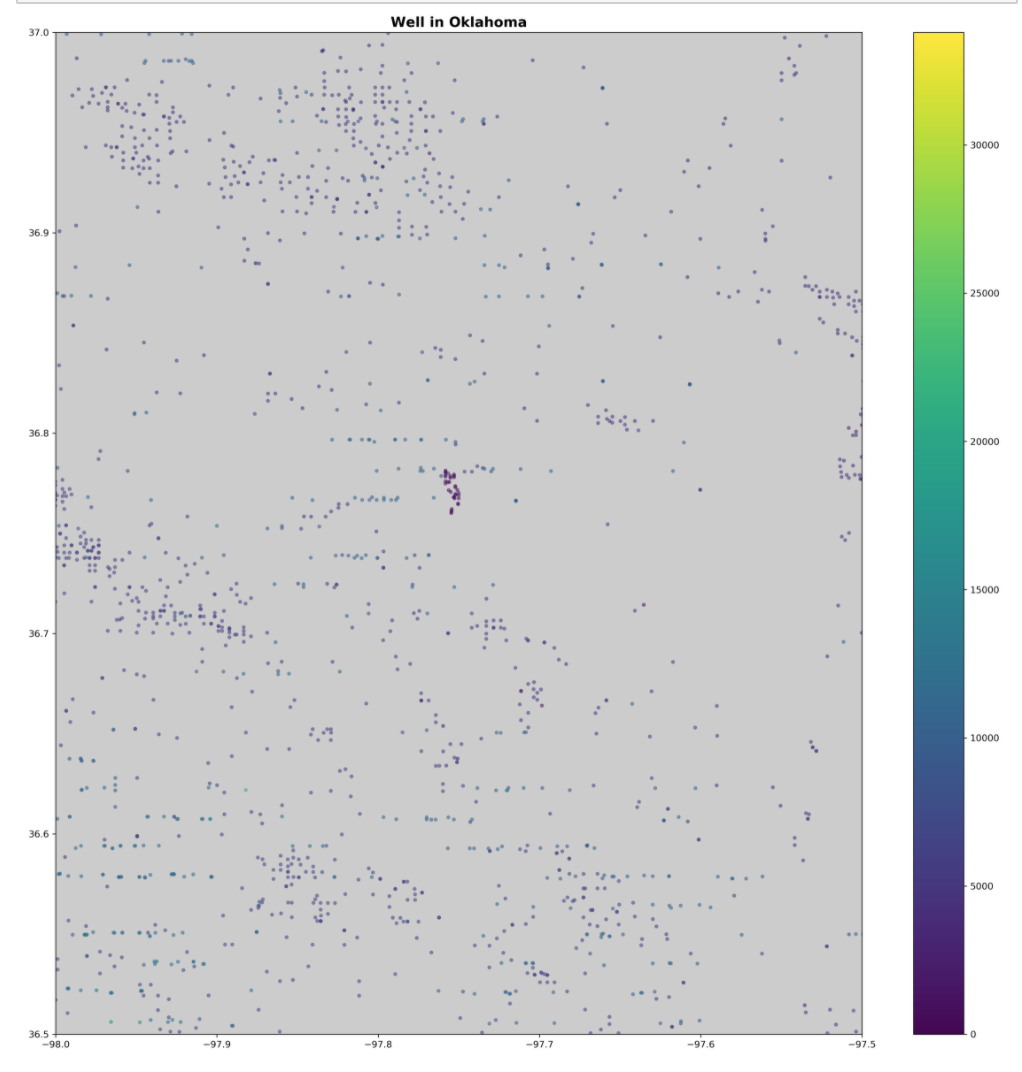
\includegraphics[scale=0.4]{well.png}
      \caption{Well Depth in Oklahoma}
      \label{fig:well}
    \end{minipage}%
    \begin{minipage}[t]{0.5\linewidth}
      \centering
      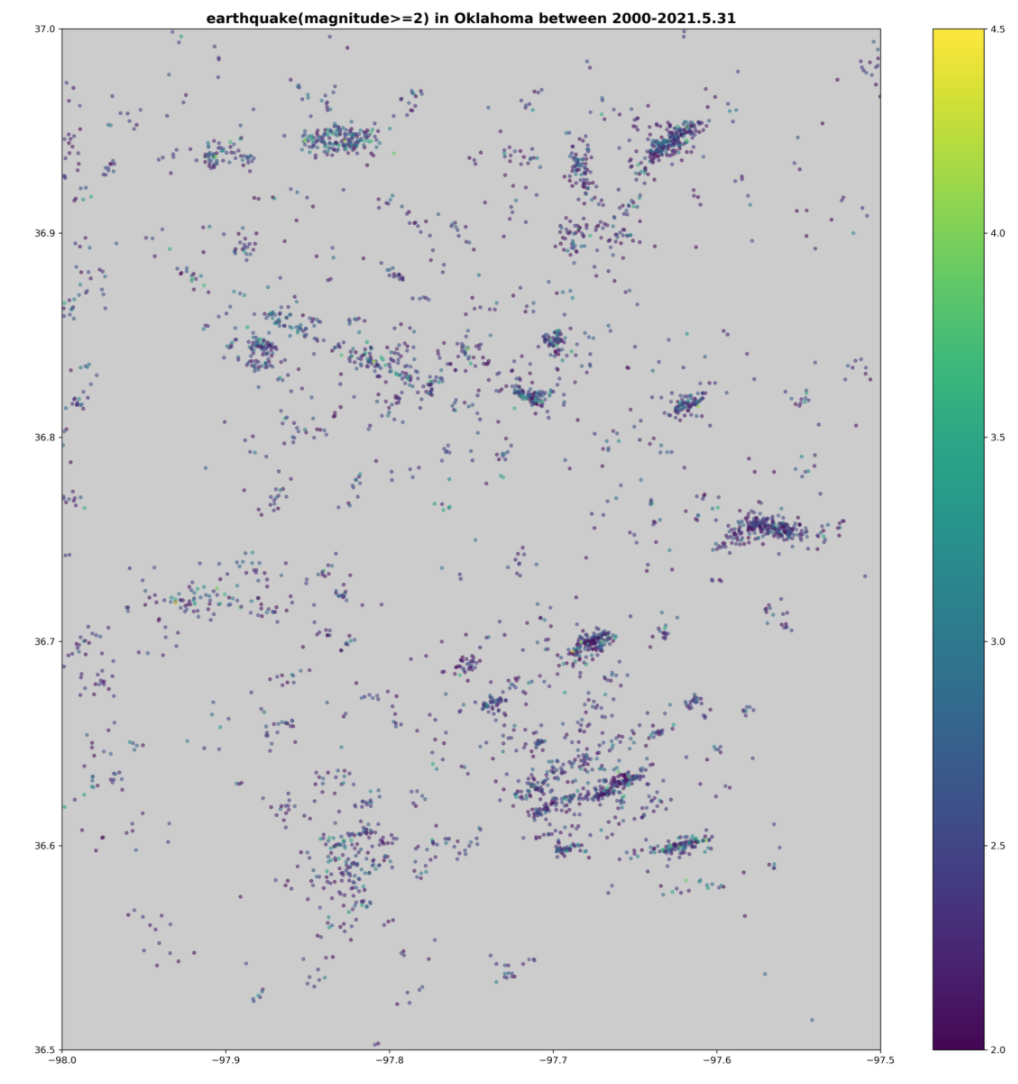
\includegraphics[scale=0.4]{earthquake.png}
      \caption{Earthquake Magnitude in Oklahoma}
      \label{fig:earthquake}
    \end{minipage}
  \end{figure}

% References
\bibliographystyle{agsm}
\bibliography{references.bib}  % BibTeX references are saved in references.bib

\clearpage
\begin{figure}
    \begin{center}
        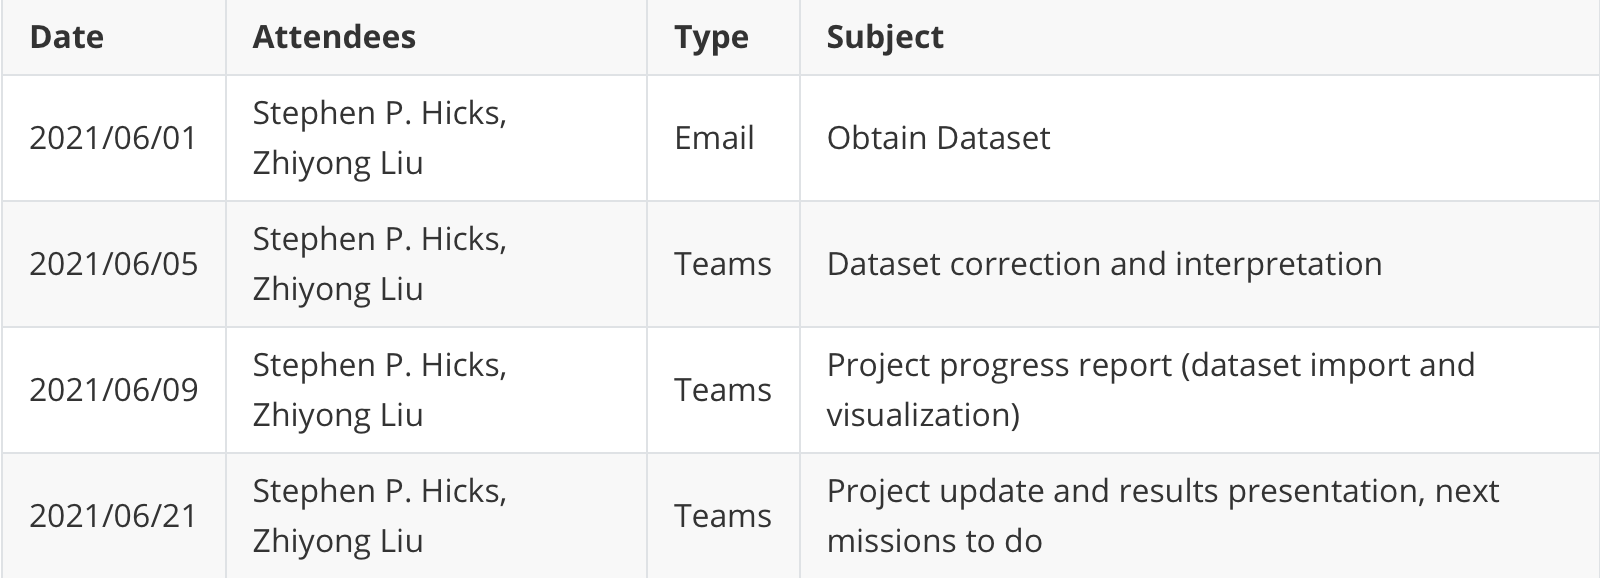
\includegraphics[width=1\textwidth]{contact.png}
    \end{center}
    \caption{\label{fig:contact} Contact Log.}
\end{figure}

\end{document}          
